% Shared by both versions: the evaluation section body (implementation,
% transaction model, exit cost, comparison, Figure 3, the batch table).

\iffullversion\else
\begin{figure}[t]
\centering
\begin{tikzpicture}
\begin{axis}[
  width=0.58\linewidth, height=\iffullversion 4.2cm\else 3.0cm\fi,
  xlabel={depth $D$ ($\log_2$ positions)}, ylabel={exit (vB)},
  xmin=7, xmax=21, ymin=0, ymax=3400,
  xtick={8,12,16,20}, grid=major, grid style={black!12},
  legend style={at={(1.04,0.5)}, anchor=west, font=\scriptsize, draw=none, fill=none, legend cell align=left, align=left},
  tick label style={font=\scriptsize}, label style={font=\scriptsize}, clip=false
]
\addplot[thick, mark=*, mark size=1.5pt] coordinates {(8,762) (12,891) (16,1020) (20,1149)};
\addlegendentry{FULL, measured}
\addplot[thick, dashed] coordinates {(8,1311) (12,1911) (16,2511) (20,3111)};
\addlegendentry{tx tree, model}
\addplot[only marks, mark=triangle*, mark size=2.2pt] coordinates {(16,1355)};
\node[font=\scriptsize, anchor=west] at (axis cs:16.4,1355) {MID 1{,}355};
\addplot[only marks, mark=diamond*, mark size=2.4pt] coordinates {(16,1473)};
\node[font=\scriptsize, anchor=east] at (axis cs:15.7,1473) {MIN 1{,}473};
\addplot[only marks, mark=square*, mark size=1.8pt] coordinates {(16,908)};
\node[font=\scriptsize, anchor=north west] at (axis cs:16.3,880) {CCV 908};
\end{axis}
\end{tikzpicture}
\caption{Exit cost against depth: LayerTree measured, radix-2 transaction tree modelled.}
\label{fig:plot}
\end{figure}
\fi

\iffullversion
\paragraph{Implementation.} A Python tapscript interpreter for both leaf
versions models BIP-441 numerics, \op{TX}, CSFS, the EC opcodes and
varops, computes the real BIP-341 signature message and enforces
\texttt{MINIMALDATA}; it models consensus limits, not standardness.
Every compiled predicate runs against a reference tree with positive and
negative cases per rule (forged leaf, stale root, attacker-chosen $m$,
unconserved amount, early eviction, voucher replay, and others): 1{,}610
FULL, 1{,}391 MID, 57 MIN and 4{,}295 CCV checks, failing if a script uses an
opcode outside its tier, plus 220 for channel leaves and 133 for the
hypothetical opcode of \S\ref{sec:discussion}. A Go implementation on
\texttt{btcd} and \texttt{lnd} generates the same scripts, byte-exact
against 145 golden scripts, and builds, signs and verifies every
transition of every tier (427 cases), each witness replayed through the
simulator; its BIP-341 signature hash equals the simulator's.
\else
\paragraph{Implementation and model.} A Python tapscript interpreter for
both leaf versions computes the real BIP-341 signature message and runs
every compiled script against a reference tree, with positive and
negative cases per rule; a Go implementation on
\texttt{btcd} and \texttt{lnd} generates the same scripts byte for byte
and builds, signs and verifies every transition of every tier. A vB figure is a
whole transaction on a $946\WU$ skeleton (Appendix~\ref{app:cmp-model}).
\fi

\iffullversion
\paragraph{The transaction model.} Every vB figure is a whole
transaction: script, witness elements and a 129-byte control block (the
eight-leaf reference script set) as measured, plus a $946\WU$ skeleton
(the tree input, a P2WPKH fee input, the tree output, one P2TR payout, a
P2WPKH change output, version, lock time and counts) and $172\WU$ per
further payout, with $\mathrm{vB} = \lceil \mathrm{WU}/4 \rceil$;
transitions without a payout (joins, updates, carves) are charged
$172\WU$ less. The witness item count and per-item length prefixes are
excluded (on a dense $D = 16$ exit, $10.5\vB$ in FULL, 10 in CCV, 42.5
in MID, 44.75 in MIN), and the baselines omit the same overhead. A deployment that carries the
sweeps, rewrites and variants needs 16 to 32 tapleaves, which adds 8 to
$16\vB$ to every spend.
\fi

\paragraph{Exit cost.} A dense exit (Figure~\ref{fig:plot},
Table~\ref{tab:sizes}) costs $762\vB$ at $D = 8$ and $1{,}149\vB$ at
$D = 20$, about $32\vB$ per level. One tier step costs as much as 10 (MID, $+33\%$, or $+36\%$
serialised) to 14 (MIN, $+44\%$, or $+47\%$) levels of depth.

\paragraph{Comparison with transaction trees.} The dashed line of
Figure~\ref{fig:plot} is a \emph{model}: an exiter publishes $D$
transactions of about $150\vB$\iffullversion{} (one key-path input, two P2TR outputs)\fi{} and
a $111\vB$ claim, anchors and their fee children omitted, which favours
the tree. LayerTree is about 60\% smaller at $D = 16$\iffullversion; a radix-4 tree
needs $2{,}031\vB$, and an Ark member of a 256-member round unrolls
$1{,}311\vB$. Under mass exit a tree's interior is shared, about $261\vB$
per member at radix 2 and $191\vB$ at radix 4 with the claim, against
$165\vB$ for a cohort leaving by \tr{REWRITE}$_6$ (Table~\ref{tab:ark},
Appendix~\ref{app:eval})\else, $165$ against $261\vB$ a member under
mass exit\fi. The model omits the latency of $D$
confirmations and the larger opcode set\iffullversion\else{}
(Appendix~\ref{app:compare})\fi.



\iffullversion
\begin{figure}[tbp]
\centering
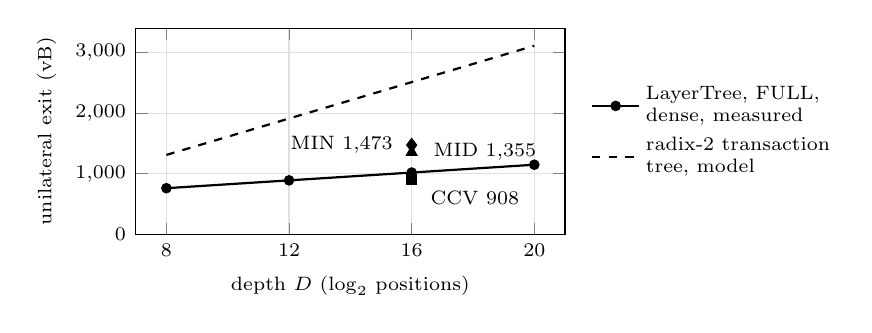
\begin{tikzpicture}
\begin{axis}[
  width=0.58\linewidth, height=4.2cm,
  xlabel={depth $D$ ($\log_2$ positions)}, ylabel={unilateral exit (vB)},
  xmin=7, xmax=21, ymin=0, ymax=3400,
  xtick={8,12,16,20}, grid=major, grid style={black!12},
  legend style={at={(1.04,0.5)}, anchor=west, font=\scriptsize, draw=none, fill=none, legend cell align=left, align=left},
  tick label style={font=\scriptsize}, label style={font=\scriptsize}, clip=false
]
\addplot[thick, mark=*, mark size=1.5pt] coordinates {(8,762) (12,891) (16,1020) (20,1149)};
\addlegendentry{LayerTree, FULL,\\dense, measured}
\addplot[thick, dashed] coordinates {(8,1311) (12,1911) (16,2511) (20,3111)};
\addlegendentry{radix-2 transaction\\tree, model}
\addplot[only marks, mark=triangle*, mark size=2.2pt] coordinates {(16,1355)};
\node[font=\scriptsize, anchor=west] at (axis cs:16.4,1355) {MID 1{,}355};
\addplot[only marks, mark=diamond*, mark size=2.4pt] coordinates {(16,1473)};
\node[font=\scriptsize, anchor=east] at (axis cs:15.7,1473) {MIN 1{,}473};
\addplot[only marks, mark=square*, mark size=1.8pt] coordinates {(16,908)};
\node[font=\scriptsize, anchor=north west] at (axis cs:16.3,880) {CCV 908};
\end{axis}
\end{tikzpicture}
\caption{Unilateral exit cost against tree depth: measured for LayerTree (FULL, and the other tiers at $D=16$), modelled for an unamortised radix-2 transaction tree.}
\label{fig:plot}
\end{figure}
\fi

\iffullversion
\paragraph{A native opcode (hypothetical).} Tapscript has no loops, so
the tiers pay for every level of a path in script, and that is the cost
they change only by a constant. A hypothetical \op{MERKLESUMUPDATE} would
take a proof, an old node and a new node and return the root of the old
node's path and the root with the new node in its place. The proof is a
depth, a position and a bitmap naming the levels that carry a sibling,
then those 40-byte siblings; every other level uses the empty node
$\Emp_k$. The opcode adds the sums, fails on overflow past $2^{64}$ or on
a non-canonical proof, and costs $2\times$ the depth in hashes, charged as
BIP-440 varops. It replaces the unrolled fold and the sum arithmetic along the path; the script that remains checks the leaf, the payout and, for a pending receive, the amounts it moves. Nobody has proposed it and nothing here depends on
it; it runs only in the simulator, behind a flag, in no tier and in no golden script.

\tr{EXIT}$_1$ then has 252 bytes of script at every depth (2{,}101 in
FULL and 1{,}716 in CCV at $D = 16$), and one 40-byte witness sibling per
occupied level. Empty levels cost nothing, so a hashed-position tree (Appendix~
ef{app:sparse}) costs about the same as a dense one. For
$2^k$ members in a key-addressed depth-64 tree the exit is about
$381 + 10k\vB$ (541 at $2^{16}$\iffullversion, 701 at $2^{32}$\fi), against $504 + 32.25k$
for FULL (1{,}020\iffullversion; 1{,}536\fi) and $150k + 111$ for a transaction tree
(2{,}511\iffullversion; 4{,}911\fi): $10\vB$ per doubling and no fixed depth.
\iffullversion Figure~\ref{fig:scale} plots this. The six-leaf
$388\vB$ of Figure~\ref{fig:anatomy} and the $520\vB$ of a full depth-16
tree are the simulator's smaller model; 541 is the key-addressed one.
\fi
The \tr{CLAIM}$^{hm}$ redemption of a pending leaf (\S\ref{sec:pending}) is
$626\vB$ at $2^{16}$ members against $1{,}136\vB$ in FULL. This and the settlement figure below assume a proof that can start above height 0 (a start-height field), or a dense tree of depth exactly $k$: the opcode's empty chain starts at $\Emp_0$, so without either a height-$h$ proof carries every empty level, about $480\vB$ more per merge or rewrite at $2^{16}$ members.

It does little for batches. A rewrite is dominated by a per-position step of about 376 bytes of script at $h = 6$, which the
opcode does not touch: settling pending receives costs $547\vB$ a pair
at 64 positions\iffullversion{} (two transactions of $8{,}347$ and
$9{,}155\vB$ at $2^{16}$ members, 24{,}065 bytes of script each against
25{,}036 in FULL)\fi. A multi-leaf exit can chain $K$ calls, each call's old root the previous call's new root; a sweep needs the subtree root of its $2^h$ leaves, which the proof format above does not express. The price is that the opcode fixes in
consensus this tree's node encoding, empty-node chain, parent hash and
overflow rule, so a different tree or a format change would need a
different opcode. That is why the work composes proposed opcodes and
proposes none, and treats the opcode as a measurement of what the
general approach pays, not as a tier (\S\ref{sec:discussion}).
\else
\paragraph{A native opcode (hypothetical).} An unproposed
\op{MERKLESUMUPDATE} would fold a Merkle-sum path in one step, replacing
the unrolled levels. \tr{EXIT}$_1$ is then 252 bytes of script at every
depth, and the exit about $381 + 10k\vB$ for $2^k$ members (541 at
$2^{16}$, against 1{,}020 for FULL and 2{,}511 for a transaction tree).
Batches gain little, since the per-position step dominates: settling
pending receives costs $547\vB$ a pair at 64 positions. It fixes this
tree's encoding in consensus, so the work treats it as a measurement, not
a tier (\S\ref{sec:discussion}, Appendix~\ref{app:native}).
\fi

\iffullversion
\begin{figure}[tbp]
\centering
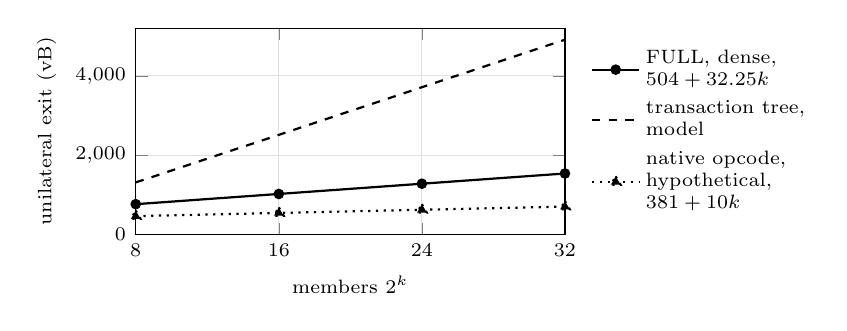
\begin{tikzpicture}
\begin{axis}[
  width=0.58\linewidth, height=4.2cm,
  xlabel={members $2^k$}, ylabel={unilateral exit (vB)},
  xmin=8, xmax=32, ymin=0, ymax=5200,
  xtick={8,16,24,32}, grid=major, grid style={black!12},
  legend style={at={(1.04,0.5)}, anchor=west, font=\scriptsize, draw=none, fill=none, legend cell align=left, align=left},
  tick label style={font=\scriptsize}, label style={font=\scriptsize}, clip=false
]
\addplot[thick, mark=*, mark size=1.5pt] coordinates {(8,762) (16,1020) (24,1278) (32,1536)};
\addlegendentry{FULL, dense,\\$504 + 32.25k$}
\addplot[thick, dashed] coordinates {(8,1311) (16,2511) (24,3711) (32,4911)};
\addlegendentry{transaction tree,\\model}
\addplot[thick, dotted, mark=triangle*, mark size=2pt] coordinates {(8,461) (16,541) (24,621) (32,701)};
\addlegendentry{native opcode,\\hypothetical,\\$381 + 10k$}
\end{axis}
\end{tikzpicture}
\caption{Exit cost against membership $2^k$ under the scaling model: a key-addressed depth-64 tree for the hypothetical native opcode, dense depth $k$ for FULL, a radix-2 transaction tree. The dotted line needs an opcode no one has proposed.}
\label{fig:scale}
\end{figure}
\fi

% The batch table (table-batch.tex) and its paragraph are the full
% version's here; the short version gives each shape in its operations
% section and carries the table in its cost appendix.
\iffullversion
% The batch-shape table, shared by both versions: the full version's
% evaluation section (body-eval.tex) and the short version's cost
% appendix (appendix-compare.tex).

\begin{table}[tbp]
\centering
\caption{Batch shapes at dense $D = 16$ on the transaction model: vB per leaf that leaves or changes, or per member that joins. Self-funded joins add each member's P2TR key-path funding input ($58\vB$) and the signing round of \S\ref{sec:parties}. The \tr{REWRITE}$_h$ rows are FULL's figures.}
\label{tab:batch}
\setlength{\tabcolsep}{4pt}\scriptsize
\begin{tabular}{@{}lrrr@{\quad}lrrr@{}}
\toprule
removal & leaves & tx & per leaf & addition or change & leaves & tx & per leaf \\
\midrule
\tr{EXIT}$_1$ & 1 & 1{,}020 & 1{,}020 & \tr{JOIN}$_0$ & 1 & 937 & 937 \\
\tr{EXIT}$_2$ & 2 & 1{,}684 & 842 & \tr{JOIN}$_2$ & 4 & 872 & 218 \\
\tr{EVICT\_SUBTREE}$_4$ & 13 & 2{,}638 & 203 & \tr{JOIN}$_8$ (operator-funded) & 256 & 679 & 2.7 \\
\tr{EVICT\_SUBTREE}$_6$ & 51 & 8{,}057 & 158 & sparse \tr{JOIN}$_0$, $D = 32$ & 1 & 1{,}601 & 1{,}601 \\
\tr{REWRITE}$_2$, all leave & 4 & 1{,}455 & 364 & \tr{REWRITE}$_6$, keys rotated & 64 & 9{,}496 & 148 \\
\tr{REWRITE}$_6$, all leave & 64 & 10{,}392 & 162 & \tr{UPDATE}, one leaf & 1 & 1{,}030 & 1{,}030 \\
\bottomrule
\end{tabular}
\end{table}


\paragraph{Batching and joins.} A second exit in the same transaction
adds $665\vB$ (its marginal weight rounded up on its own, one more than
$1{,}684 - 1{,}020$), against $158$ to $165\vB$ per leaf for a sweep or
a rewrite (Table~\ref{tab:batch}). A graft
costs the operator under $3\vB$ per member, so a self-funded member's own
input dominates its entry. Off-chain, a member follows every spend of the
tree output (about 1\,kB of witness each), and the operator stores the
whole tree.
\fi

\iffullversion
\paragraph{Fees and budgets.} At $10\sat/\mathrm{vB}$ a $D=16$ exit
costs $10{,}200\sat$, a 1\% fee on $1{,}020{,}000\sat$
(Appendix~\ref{app:eval}). Varops usage is 5.6 to 7.7\% of the BIP-440
budget in the dense profile, falling with depth because the budget scales with weight;
\texttt{0xC0} tiers use one to three signature operations of the BIP-342
sigop budget.
\fi

\iffullversion
\paragraph{Artefact.} Every number here is regenerated from the
repository~\cite{layertreerepo} at the revision on the title page
(\GitHash) by the scripts under \path{tools/}: \path{test_scripts.py}
(1{,}610 checks; \texttt{-{}-rewrite} and \texttt{-{}-subtree} print the
cohort shapes), \path{test_mid.py} (1{,}391), \path{test_min.py} (57),
\path{test_ccv.py} (4{,}295), \path{test_chan.py} (220), \path{test_msu.py}
(133), \path{gen_listings.py} (the size table), \path{fee_analysis.py}
(the fee model), \path{gen_golden.py} and \path{experiments/radix4.py}
(55); by \texttt{go test ./...}; and by \texttt{lake build} in
\path{formal/}, which prints the axiom audit. Figure coordinates are
copied from these outputs by hand.
\fi
